%!TEX root = ../../tcc.tex

\subsection*{Mensagens}

O protocolo é definido por doze mensagens e dois tipos de assinaturas. Essas mensagens
são enviadas entre \glspl*{peer} e servem para estes tomarem conhecimento da situação de
download de um \gls*{torrent}. A primeira assinatura é exclusiva da mensagem de
\emph{handshake}, enquanto todas as outras seguem o mesmo padrão.

\subsubsection*{handshake}

assinatura: \bverb|<tam. header><header><bytes reservados><info_hash><peer_id>|

O \emph{handshake} (aperto de mãos) é a primeira mensagem a ser enviada por um
\gls*{peer} recém-chegado à rede:

\begin{description}
    \item[<tam. header>:] tamanho da string \bverb|<header>|, representado em binário
        por 1 byte. O comprimento oficial é 19.

    \item[<header>:] \gls*{string} identificadora do protocolo. Na versão 1.0 do
        protocolo BitTorrent, a \gls*{string} oficial é \sverb|BitTorrent protocol|.

    \item[<bytes reservados>:] seção de 8 bytes (= 64 bits) reservados para a
        habilitação de funcionalidades extras do protocolo. Um e-mail enviado pelo
        criador do BitTorrent, Bram Cohen \cite{wikitheory:reserved-bytes}, sugere que
        os bits menos significativos sejam usados primeiro, para que os mais
        significativos possam ser usados para alterar o significado dos bits finais. A
        implementação de cada uma das funcionalidades não-oficiais depende do programa
        cliente. A tabela abaixo mostra os bits e seus respectivos usos, oficiais (*)
        e não-oficiais.

        \begin{center}
            \begin{tabular}{ | c | c |}
            \hline
            \textbf{Bit} & \textbf{Uso}                         \\ \hline
            1       & Azureus Extended Messaging                \\ \hline
            1-16    & BitComet Extension protocol               \\ \hline
            21      & BitTorrent Location-aware Protocol 1.0    \\ \hline
            44      & Extension protocol                        \\ \hline
            47-48   & Extension Negotiation Protocol            \\ \hline
            61      & NAT Traversal                             \\ \hline
            62      & Fast Peers*                               \\ \hline
            63      & XBT Peer Exchange                         \\ \hline
            64      & DHT* ou XBT Metadata Exchange             \\ \hline
            \end{tabular}
        \end{center}

    \item[<info_hash>:] o ID do \gls*{torrent}, que é a \gls*{string}
        \gls*{hashvalue} de 20 bytes resultante da \gls*{hashfunction} SHA-1, com
        \gls*{urlencode}, do valor da chave \bverb|info| do \gls*{torrentfile}; e

    \item[<peer_id>:] ID único do cliente, que é uma \gls*{string} de 20 bytes,
        geralmente sendo o mesmo valor \bverb|peer_id| enviado nas requisições ao
        \gls*{tracker}, prefixado pelas informações do nome do programa cliente e de sua
        versão (o Transmission envia o prefixo \sverb|-TR2820-...|).
\end{description}

\cfile[label="./libtransmission/handshake.c:191"]{./Codes/chap3/028-handshake.c}

Essa mensagem é enviada imediatamente pelo \gls*{peer} que inicia uma conexão. O
receptor deve responder com o seu \bverb|peer_id|, assim que detectar o ID do
\gls*{torrent} na seção de \bverb|info_hash| da mensagem. A conexão deve ser fechada em
dois casos: pelo receptor, se ele receber a mensagem para um ID de \gls*{torrent}
desconhecido para si; ou pelo iniciador, caso o \bverb|peer_id| recebido como resposta
seja diferente daquele indicado na lista de \glspl*{peer} recebida do \gls*{dht}.

\subsubsection*{keep-alive}

keep-alive: \bverb|<tamanho=0000>|

A mensagem de \emph{keep-alive} (``mantenha vivo'', em português literal) serve para
manter uma conexão aberta, caso nenhuma outra mensagem seja enviada num determinado
período de tempo (geralmente, dois minutos).

Assim como as mensagens que serão descritas a seguir, esta mensagem usa a assinatura:

\bverb|<tamanho><ID da mensagem><dados>|

\begin{description}
    \item[<tamanho>:] valor de 4 bytes em \emph{big} \gls{endian};

    \item[<ID da mensagem>:] decimal de 1 byte; e

    \item[<dados>:] dados a serem enviados ao outro \gls*{peer}, dependente da
        mensagem.
\end{description}

Porém, não possui ID da mensagem nem dados a serem enviados, apresentando tamanho 0.

\cfile[label="./libtransmission/peer-msgs.c:1093"]{./Codes/chap3/029-keepalive.c}

\subsubsection*{choke e unchoke}

\hspace*{-\parindent} % alinha a tabela à margem esquerda
\begin{tabular}{r l}
\textbf{choke:} & \bverb|<tamanho=0001><ID da mensagem=0>| \\
\textbf{unchoke:} & \bverb|<tamanho=0001><ID da mensagem=1>|
\end{tabular}

Estas mensagens servem para indicar a mudança de estado de choking (ou estrangulamento)
da conexão (a maneira que o \gls*{peer} remetente tratará o receptor). Ou seja, o
receptor ``estrangulado'' (ou \emph{choked}) não terá suas requisições atendidas, ao
contrário de quando estiver com sua conexão livre (ou \emph{unchoked}).

\cfile[label="./libtransmission/peer-msgs.c:431"]{./Codes/chap3/030-choke-unchoke.c}

\subsubsection*{interested e not interested}

\hspace*{-\parindent} % alinha a tabela à margem esquerda
\begin{tabular}{r l}
\textbf{interested:} & \bverb|<tamanho=0001><ID da mensagem=2>| \\
\textbf{not interested:} & \bverb|<tamanho=0001><ID da mensagem=3>|
\end{tabular}

Estas duas mensagens também servem para indicar mudança de estado, mas no sentido de
mudança de interesse que o \gls*{peer} remetente terá no receptor.

\cfile[label="./libtransmission/peer-msgs.c:769"]{./Codes/chap3/031-interest.c}

\subsubsection*{have}

\textbf{have:} \bverb|<tamanho=0005><ID da mensagem=4><dados=i-ésima parte>|

A definição é que esta mensagem avisa um \gls*{peer} que a $i$-ésima parte do
\gls*{torrent} foi baixada pelo remetente, e verificada através de \gls*{hashvalue}.
Porém, não necessariamente é usada dessa forma.

\cfile[label="./libtransmission/peer-msgs.c:399"]{./Codes/chap3/032-have.c}

Uma implementação de algoritmo do jogo da troca pode fazer com que um \gls*{peer}, que
acabou de adquirir a parte, não emita aviso para todos os \glspl*{peer} vizinhos que já
possuem. Isso diminui a quantidade total de mensagens enviadas, contribuindo para a
redução do \gls{overhead} do protocolo. Por outro lado, enviar esse aviso pode ajudar
na determinação de qual parte é mais rara.

\subsubsection*{bitfield}

\textbf{bitfield:} \bverb|<tamanho=0001+X><ID da mensagem=5><dados=mapa de bits>|

O BitTorrent usa bitfields (mapas de bits), em \emph{big} \gls*{endian}, para
representar (em forma de bits sinalizadores) quais partes de um \gls*{torrent} já
possui.

Esta mensagem deve ser enviada imediatamente após o processo de \emph{handshake}
terminar, e antes de qualquer outra mensagem. Se o \gls*{peer} não tiver nenhuma parte,
o campo de dados pode ser omitido. Como bitfields variam de acordo com o tamanho total
do \gls*{torrent}, o comprimento da mensagem é variável, onde $X$ é o comprimento do
bitfield, acrescentado de alguns bits 0 de sobra (\emph{spare bits}) no seu final.

Bitfields de comprimento errado, ou sem bits de sobra no final, são considerados erros,
e as respectivas conexões devem ser fechadas.

\cfile[label="./libtransmission/peer-msgs.c:2120"]{./Codes/chap3/033-bitfield.c}

\subsubsection*{request}

\textbf{request:} \bverb|<tamanho=0013><ID da mensagem=6><dados=<índice><início><tamanho>>|

Conforme foi explicado anteriormente (página \pageref{subsec:partes}), um
\gls*{torrent} divide os dados em partes, que por sua vez são divididas em blocos, que
são os conteúdos trocados entre os \glspl*{peer}. Assim, o tamanho das partes é um
múltiplo do tamanho dos blocos.

\begin{figure}[H]
    \centering
    \fbox{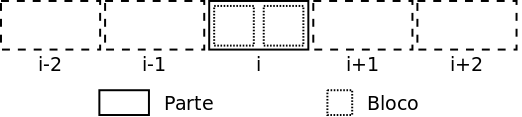
\includegraphics[width=0.64\textwidth]{partes.png}}
    \caption{trecho da seção de dados do torrent, com as divisões das partes e dos
    blocos}
    \label{fig:partes}
\end{figure}

Com esta mensagem, um \gls*{peer} pede por uma parte do \gls*{torrent}. A seção de dados
contém os seguintes números inteiros:

\begin{figure}[ht!]
    \centering
    \fbox{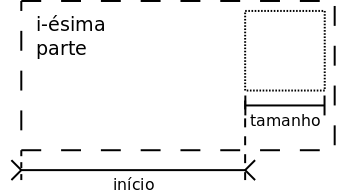
\includegraphics[width=0.64\textwidth]{request.png}}
    \caption{parâmetros da mensagem \emph{request} e seus significados}
    \label{fig:request}
\end{figure}

\begin{description}
    \item[índice:] índice da parte base $i$;
    \item[início:] deslocamento, em bytes, da posição do bloco da parte $i$ pedida; e
    \item[tamanho:] tamanho, em bytes, do bloco pedido.
\end{description}

\cfile[label="./libtransmission/peer-msgs.c:356"]{./Codes/chap3/037-request.c}

\subsubsection*{piece}

\textbf{piece:} \bverb|<tamanho=0009+X><ID da mensagem=7><dados=<índice><início><bloco>>|

Esta mensagem é a resposta para a requisição de um bloco por meio da mensagem
\emph{request}, tendo assinatura análoga, com exceção do trecho com os dados do bloco.
Assim, um \gls*{peer} envia um bloco de dados a outro.

\newpage
O tamanho da mensagem é variável, onde $X$ é o tamanho do segmento de dados, já que
este pode ter tamanhos diferentes entre mensagens diferentes. A seção de dados possui
os seguintes números inteiros:

\begin{description}
    \item[índice:] índice da parte base $i$;
    \item[início:] deslocamento, em bytes, da posição do bloco da parte $i$ pedido; e
    \item[bloco:] conteúdo dos dados do bloco.
\end{description}

\cfile[label="./libtransmission/peer-msgs.c:1093"]{./Codes/chap3/034-piece.c}

\newpage
\subsubsection*{cancel}

\textbf{cancel:} \bverb|<tamanho=0013><ID da mensagem=8><dados=<índice><início><tamanho>>|

A mensagem \emph{cancel} serve para cancelar a mensagem \emph{request} de mesmos
parâmetros. É mais utilizada durante o algoritmo de fim de jogo (página
\pageref{subsubsec:endgame}).

\cfile[label="./libtransmission/peer-msgs.c:372"]{./Codes/chap3/035-cancel.c}

\subsubsection*{port}

\textbf{port:} \bverb|<tamanho=0003><ID da mensagem=9><dados=porta>|

Para casos em que o \gls*{peer} estiver usando a função de \gls*{dht}, esta mensagem
serve para avisar ao receptor qual a porta de comunicação \gls*{tcp} é usada pelo
remetente para receber mensagens de \gls*{dht}. Com isso, é adicionado à tabela de
roteamento do receptor.

\cfile[label="./libtransmission/peer-msgs.c:387"]{./Codes/chap3/036-port.c}
